\section{Simulation folder structure}

All \swdd project folders must obey a specific structure, otherwise leading to runtime errors. For a complete run (from scratch) a project folder must contain 2 folders. Then, after the \swConverter and \swSolver executables have been run, the project folder contains 4 folders (see Figure \ref{fig:simu_tree}) : \\
%\includegraphics[width=3.5cm]{../common/figures/simu_tree}

\begin{figure}[htbp]
    \centering
    
\includegraphics[width=3.5cm]{../../common/figures/simu_tree_before.png}\;\;\;   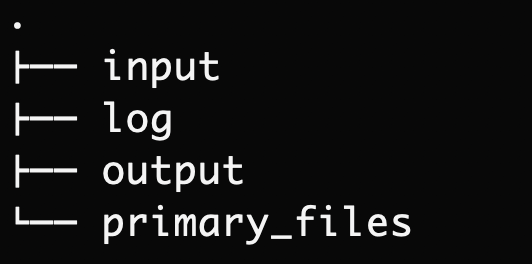
\includegraphics[width=3.5cm]{../../common/figures/simu_tree_after.png}
    \caption{Project folder tree before (left) and after (right) the \swConverter + \swSolver sequence is run.}
    \label{fig:simu_tree}
\end{figure}

\begin{description}
	\item [input] folder containing the input files. This folder is needed to run \swSolver. \	\item [log]  This folder contains the log files allowing to trace the computation process. If the folder does not exists prior to a new simulation, it is created by \swSolver. If the folder exists at the beginning of a simulation, the previous content is deleted.
	\item [log] This folder contains log files (mostly regarding mesh properties and console logs).
	\item [output] This folder contains the simulation results in an user-readable (text) and/or binary format. If the folder does not exists prior to a new simulation, it is created by \swSolver. If the folder exists at the beginning of a simulation, the previous content is deleted.
	\item [primary\_files] This folder contains the files necessary to construct \file{geometry.sw2d}. It is compulsory for running \swConverter but  not used by \swSolver. Since the content of this folder is not deleted by the program, the user can store complementary files.
\end{description}




